\documentclass[]{article}
\usepackage{lmodern}
\usepackage{amssymb,amsmath}
\usepackage{ifxetex,ifluatex}
\usepackage{fixltx2e} % provides \textsubscript
\ifnum 0\ifxetex 1\fi\ifluatex 1\fi=0 % if pdftex
  \usepackage[T1]{fontenc}
  \usepackage[utf8]{inputenc}
\else % if luatex or xelatex
  \ifxetex
    \usepackage{mathspec}
  \else
    \usepackage{fontspec}
  \fi
  \defaultfontfeatures{Ligatures=TeX,Scale=MatchLowercase}
\fi
% use upquote if available, for straight quotes in verbatim environments
\IfFileExists{upquote.sty}{\usepackage{upquote}}{}
% use microtype if available
\IfFileExists{microtype.sty}{%
\usepackage{microtype}
\UseMicrotypeSet[protrusion]{basicmath} % disable protrusion for tt fonts
}{}
\usepackage[margin=1in]{geometry}
\usepackage{hyperref}
\hypersetup{unicode=true,
            pdftitle={Assessing Amazon turker and automated machine forecasts in the Hybrid Forecasting Competition},
            pdfauthor={Andreas Beger and Michael D. Ward},
            pdfborder={0 0 0},
            breaklinks=true}
\urlstyle{same}  % don't use monospace font for urls
\usepackage{longtable,booktabs}
\usepackage{graphicx,grffile}
\makeatletter
\def\maxwidth{\ifdim\Gin@nat@width>\linewidth\linewidth\else\Gin@nat@width\fi}
\def\maxheight{\ifdim\Gin@nat@height>\textheight\textheight\else\Gin@nat@height\fi}
\makeatother
% Scale images if necessary, so that they will not overflow the page
% margins by default, and it is still possible to overwrite the defaults
% using explicit options in \includegraphics[width, height, ...]{}
\setkeys{Gin}{width=\maxwidth,height=\maxheight,keepaspectratio}
\IfFileExists{parskip.sty}{%
\usepackage{parskip}
}{% else
\setlength{\parindent}{0pt}
\setlength{\parskip}{6pt plus 2pt minus 1pt}
}
\setlength{\emergencystretch}{3em}  % prevent overfull lines
\providecommand{\tightlist}{%
  \setlength{\itemsep}{0pt}\setlength{\parskip}{0pt}}
\setcounter{secnumdepth}{0}
% Redefines (sub)paragraphs to behave more like sections
\ifx\paragraph\undefined\else
\let\oldparagraph\paragraph
\renewcommand{\paragraph}[1]{\oldparagraph{#1}\mbox{}}
\fi
\ifx\subparagraph\undefined\else
\let\oldsubparagraph\subparagraph
\renewcommand{\subparagraph}[1]{\oldsubparagraph{#1}\mbox{}}
\fi

%%% Use protect on footnotes to avoid problems with footnotes in titles
\let\rmarkdownfootnote\footnote%
\def\footnote{\protect\rmarkdownfootnote}

%%% Change title format to be more compact
\usepackage{titling}

% Create subtitle command for use in maketitle
\newcommand{\subtitle}[1]{
  \posttitle{
    \begin{center}\large#1\end{center}
    }
}

\setlength{\droptitle}{-2em}

  \title{Assessing Amazon turker and automated machine forecasts in the Hybrid
Forecasting Competition}
    \pretitle{\vspace{\droptitle}\centering\huge}
  \posttitle{\par}
    \author{Andreas Beger and Michael D. Ward}
    \preauthor{\centering\large\emph}
  \postauthor{\par}
      \predate{\centering\large\emph}
  \postdate{\par}
    \date{2018-12-05}

\usepackage[T1]{fontenc}

\begin{document}
\maketitle
\begin{abstract}
\noindent The Hybrid Forecasting Competition (HFC) is an ongoing project
to develop hybrid geopolitical forecasting systems that combine human-
and machine-generated forecasts. The first project trial period took
place in 2018, during the course of which volunteer participants, Amazon
Mechanical Turkers, and an automated time series forecasting module we
developed provided forecasts for more than 150 questions covering a
diverse set of topics. We investigate two questions: (1) how does the
performance of turker forecasters compare to volunteers, and (2) what
impact did access to the machine forecasts have on forecaster accuracy?
\newline \newline
\end{abstract}

The Hybrid Forecasting Competition (HFC)\footnote{\textbf{Funding
  acknowledgement}: This research is based upon work supported in part
  by the Office of the Director of National Intelligence (ODNI),
  Intelligence Advanced Research Projects Activity (IARPA), via
  2017-17071900005. The views and conclusions contained herein are those
  of the authors and should not be interpreted as necessarily
  representing the official policies, either expressed or implied, of
  ODNI, IARPA, or the U.S. Government. The U.S. Government is authorized
  to reproduce and distribute reprints for governmental purposes
  notwithstanding any copyright annotation therein.} is an IARPA program
that seeks to develop methods for hybrid geopolitical forecasting system
that combine human and machine forecasts to answer a broad range of
questions about economic, political, health, and other events and
trends. The first trial period, or RCT, took place in 2018, during the
course of which hundreds of volunteer and Amazon Mechnial Turk
forecasters, as well as automated machine models, answered more than 150
questions covering a broad range of issues.

We worked on one of the competition teams, and specifically by
contributing a time series forecasting module. Out of the large set of
interesting questions one could examine with the results so far, given
our specific focus on this project, we will try to examine in this paper
two questions: (1) how does the accuracy of turker forecasters compare
to volunteer forecasters, and (2) what was the impact of the machine
forecasts on human forecaster accuracy?

\section{The Hybrid Forecasting
Competition}\label{the-hybrid-forecasting-competition}

The goal of the HFC is to find ways to optimally combine human and
machine forecasts. For example, machine forecasts can be reliable and
scalable, but are constrained by available data, idiosyncratic
questions, and cold start problems when a corpus of historical data is
not available. Human-generated forecasts on the other hand are more
flexible, but also more costly to scale and subject to various cognitive
biases.(e.g. Kahneman and Egan 2011).

The competition is organized around Good Judgement-style forecasting
tournaments (P. Tetlock 2005, P. E. Tetlock, Mellers, and Scoblic
(2017)), where forecasters answer and are scored on a diverse pool of
questions. Examples from the first trial period, RCT-A, include:

\begin{itemize}
\tightlist
\item
  What will be the long-term interest rate for South Africa (ZAF) in
  July 2018?
\item
  How many deaths perpetrated by Boko Haram will the Council on Foreign
  Relations report for June 2018?
\item
  What will be the daily closing spot price of Brent crude oil (USD per
  barrel) on 31 May 2018, according to the U.S. EIA?
\end{itemize}

Each question includes 2 to 5 answer options to which forecasters must
assign weights summing to 1. Performance for a single forecast is then
based on an ordered multinomial Brier score.

In addition to this basic ``human forecaster'' tournament, competitors
were expected to implement features that would in some fashion or
agument these human forecasts with machine-generated tools and
forecasts. An explicity requirement for the latter is that they are
automated systems, e.g.~an ad-hoc hand-tuned and expert-implemented
machine model to forecast on a question would not be allowed, rather it
would have to be a system that can generate such a model. On the other
hand, if a forecaster has the skills and inclination to use data and
model as a forecasting tool, that is perfectly allowed.

\subsection{SAGE approach}\label{sage-approach}

One of the distinguishing features of our team's approach was a system
that could automatically associate some of the RCT-A questions with a
clearly corresponding time series and display these to a forcaster. This
is based on a data platform which automatically collects and updates
data from a variety of sources, and which can associate questions, based
on their title, to an appropriate transformation of a data set if it is
in the platform and matches a known, pre-specified pattern or template.
If data is found for a question, it can then be shown to users as a
simple time series chart accompanying the relevant question.

Additionally, we could use the time series to generate a machine
forecast based on a univariate ARIMA model, and which then would either
be shown to a user, and/or submitted seperately as a standalone
forecast. The module generating these forecasts, ``basil-ts'', was based
on the Auto ARIMA model in Hyndman and Khandakar (2008), which consists
of a ARIMA-family model with an automated algorithm for determining a
reasonble specific model structure, e.g.~whether and how many
differencing orders to apply, AR and MA orders, and some other
parameters. This is wrapped in additional functionality needed to meet
the automation requirements, e.g.~recognizing how far a forecast needs
to extend, data pre-processing, converting time series to answer option
forecasts, updating forecasts with additional information if available,
etc.

\subsection{Research design for RCT-A}\label{research-design-for-rct-a}

Since the scientific goal of HFC is to evaluate various hybrid
forecasting techniques, the pripmary aspect of our research design for
RCT-A was designed to assess what impact exposure to the time series
charts and model forecasts would have on human forecaster accuracy.
Incoming forecasters were assigned to one of three experimental
conditions. The first group, A, served as control group and only had
access to a basic version of the online platform showin the question
information and tools to enter weights for the answer options. The
second group, B, could also see the time series charts, and the third
group, C, could see the chart and machine forecast. All forecasters,
regardless of group, were forecasting on the same set of questions.

There were elements in the research design to assess other design
choices but they are not relevant to the set of questions we seek to
examine here, thus we will not discuss them.

\begin{longtable}[]{@{}ll@{}}
\caption{Summary of original research design.
\label{tab:original-design}}\tabularnewline
\toprule
Condition & Treatment\tabularnewline
\midrule
\endfirsthead
\toprule
Condition & Treatment\tabularnewline
\midrule
\endhead
A & None; control\tabularnewline
B & Chart\tabularnewline
C & Chart and machine forecast\tabularnewline
\bottomrule
\end{longtable}

Comparison of groups A and B should have shown the effect of seeing a
time series chart, and of groups B and C for the effect of seeing a
model forecast. In practice, there were issues that complicated the
effective design or forecaster groupings and treatments:

\begin{itemize}
\tightlist
\item
  \textbf{Amazon Mechanical Turk forecasters}. Due to lower than
  expected activity levels, turker forecasters started to be provided
  several weeks intot he first trial period. Given activity levels at
  that time, a decision was made to assign turkers to either condition A
  or C, but not B. This mean that the group whose treatment was to only
  see charts (B) consisted only of volunteers, while the other two
  groups contained mixed populations of volunteers and turkers, thus
  adding a confounding factor for assessing the impact of charts and
  machine models.
\item
  \textbf{Gaps in data and machine coverage}. Only about 1/3 of IFPs had
  time series data available, meaning that within each condition group,
  most questions did not have a chart nor model. There was also a small
  number of instances where data was available, but a machine forecast
  was not. One example were questions related to FluNet influenza case
  counts, where a change in the data source broke the ability to update
  chart data, which would have required models to forecast over
  excessive time horizons. Since the availability of data was related to
  the type of question, it is not possible to rule out the possibility
  that questions with data were systematically different in their
  difficulty from questions without data.
\item
  \textbf{Changes in the data and machine forecasting platforms over
  time}. Both the data platform and the machine forecasting system
  suffered from various bugs and related issues, especially during the
  earlier portions of RCT-A. These problems in some cases resulted in
  incorrectly aggregated or otherwise inaccurate data, insufficient
  updating which led to data in the platform falling behind source
  availability and thus requiring forecasts over longer time periods
  than neccessary, and bugs in the machine forecaster that led to no or
  bad forecasts. The quality of the data and machine forecasts displayed
  to some users thus varied over time and IFPs, in ways that are
  difficult to reconstruct in retrospective.
\end{itemize}

In respect to the first two problems, which we can quantify, the
effective treatment groups were more complicated and are showin in Table
\ref{tab:all-conditions}.

\begin{longtable}[]{@{}rlllll@{}}
\caption{Effective treatments by group after addition of turkers to
conditions A and C. \label{tab:all-conditions}}\tabularnewline
\toprule
Group & Condition & Forecaster & IFP\_Group & Sees chart? & Sees
model?\tabularnewline
\midrule
\endfirsthead
\toprule
Group & Condition & Forecaster & IFP\_Group & Sees chart? & Sees
model?\tabularnewline
\midrule
\endhead
1 & A: no chart & Turker & No TS data & &\tabularnewline
2 & A: no chart & Turker & Chart only & &\tabularnewline
3 & A: no chart & Turker & Chart and model & &\tabularnewline
4 & A: no chart & Volunteer & No TS data & &\tabularnewline
5 & A: no chart & Volunteer & Chart only & &\tabularnewline
6 & A: no chart & Volunteer & Chart and model & &\tabularnewline
7 & B: chart only & Volunteer & No TS data & &\tabularnewline
8 & B: chart only & Volunteer & Chart only & X &\tabularnewline
9 & B: chart only & Volunteer & Chart and model & X &\tabularnewline
10 & C: chart and model & Turker & No TS data & &\tabularnewline
11 & C: chart and model & Turker & Chart only & X &\tabularnewline
12 & C: chart and model & Turker & Chart and model & X &
X\tabularnewline
13 & C: chart and model & Volunteer & No TS data & &\tabularnewline
14 & C: chart and model & Volunteer & Chart only & X &\tabularnewline
15 & C: chart and model & Volunteer & Chart and model & X &
X\tabularnewline
16 & Machine & Machine & Chart and model & &\tabularnewline
\bottomrule
\end{longtable}

\section{Design, data, and method}\label{design-data-and-method}

\subsection{DGP}\label{dgp}

Question comes from T\&E to our platform.

Now on two tracks:

\begin{enumerate}
\def\labelenumi{\arabic{enumi}.}
\tightlist
\item
  Human
\end{enumerate}

\begin{itemize}
\tightlist
\item
  sees question, and depending on condition the chart and machine
  forecast
\item
  forecasts, possibly multiple times per day
\item
  Mean daily Brier score
\end{itemize}

\begin{enumerate}
\def\labelenumi{\arabic{enumi}.}
\setcounter{enumi}{1}
\tightlist
\item
  Platform
\end{enumerate}

\begin{itemize}
\tightlist
\item
  parses question, finds associated data
\item
  sends question and data to forecaster
\item
  forecaster parses question and data, TS forecast, convert to MN
  forecast
\item
  mean daily Brier score and/or shown to user
\end{itemize}

\subsection{Data}\label{data}

RCT-A lasted from March 7th to September 7th 2018. However, Turkers did
not enter until May 2nd, and for an unrelated reason we also discard
data after August 2nd. This leaves a total of 48,931 forecasts---7,816
from volunteer forecasters, 39,140 from Turkers, and 1,975 from
machine---for 156 IFPs, of which 101 did not have TS data, 6 had TS data
but not a machine forecast, and 49 had both TS data and a machine
forecast.

\section{Results}\label{results}

\begin{table}

\caption{\label{tab:brier-by-forecaster}Average Brier score by forecaster group}
\centering
\begin{tabular}[t]{lrr}
\toprule
Forecaster & avg\_Brier & n\\
\midrule
Machine & 0.39 & 1975\\
Turker & 0.43 & 39140\\
Volunteer & 0.32 & 7816\\
\bottomrule
\end{tabular}
\end{table}

Volunteers who had only charts did the best

\begin{table}

\caption{\label{tab:brier-by-forecaster-condition}Average Brier score by forecaster group}
\centering
\begin{tabular}[t]{lrrrr}
\toprule
Forecaster & A: no chart & B: chart only & C: chart and model & Machine\\
\midrule
Machine &  &  &  & 0.39\\
Turker & 0.44 &  & 0.43 & \\
Volunteer & 0.30 & 0.25 & 0.37 & \\
\bottomrule
\end{tabular}
\end{table}

Table \ref{tab:brier-by-forecaster-ifp-group-condition} summarizes the
average Brier scores for all 16 treatment/forecaster/IFP groups in Table
XX. As it is quite unwieldy, we include it for reference and will
discuss specific insights in more details below.

\begin{table}

\caption{\label{tab:brier-by-forecaster-ifp-group-condition}Average Brier scores for all 15 distinct human IFP/treatment groups, as well as the machine forecasts}
\centering
\begin{tabular}[t]{rlllrrr}
\toprule
Group & Condition & Forecaster & IFP\_Group & avg\_Brier & sd\_Brier & n\\
\midrule
1 & A: no chart & Turker & No TS data & 0.45 & 0.50 & 6690\\
2 & A: no chart & Turker & Chart only & 0.55 & 0.56 & 304\\
3 & A: no chart & Turker & Chart and model & 0.39 & 0.40 & 2907\\
4 & A: no chart & Volunteer & No TS data & 0.31 & 0.54 & 510\\
5 & A: no chart & Volunteer & Chart only & 0.36 & 0.46 & 18\\
6 & A: no chart & Volunteer & Chart and model & 0.28 & 0.34 & 274\\
\addlinespace
7 & B: chart only & Volunteer & No TS data & 0.26 & 0.48 & 1702\\
8 & B: chart only & Volunteer & Chart only & 0.42 & 0.42 & 57\\
9 & B: chart only & Volunteer & Chart and model & 0.23 & 0.31 & 973\\
\addlinespace
10 & C: chart and model & Turker & No TS data & 0.45 & 0.50 & 19502\\
11 & C: chart and model & Turker & Chart only & 0.56 & 0.52 & 990\\
12 & C: chart and model & Turker & Chart and model & 0.38 & 0.40 & 8747\\
13 & C: chart and model & Volunteer & No TS data & 0.38 & 0.60 & 3090\\
14 & C: chart and model & Volunteer & Chart only & 0.59 & 0.57 & 73\\
15 & C: chart and model & Volunteer & Chart and model & 0.32 & 0.40 & 1119\\
16 & Machine & Machine & Chart and model & 0.39 & 0.36 & 1975\\
\bottomrule
\end{tabular}
\end{table}

\subsection{Turkers generally did
worse}\label{turkers-generally-did-worse}

Turkers overall had worse forecast accuracy than either the machine
models or volunteers. To rule a spurious relationship, we can compare
the accuracy in directly comparable pairs, e.g.~rows 1 and 4 in Table
\ref{tab:brier-by-forecaster-ifp-group-condition} consists of the
average Brier scores for questions without TS data and in condition A
treatment group for turkers and volunteers respectively, and show a
difference of 0.14.

Figure \ref{fig:turkers} shows the results of pairwise comparisons of
the average Brier scores for all groups relative to Turker forecasters.
Each row in the plot corresponds to a linear model for forecasters from
the corresponding condition and IFP group, and the pointranges show
coefficient estimates and 95\% confidence intervals for Turkers,
Machine, and Volunteer forecasters. The Turker values correspond to the
average Brier for them in this grouping, while the Machine and Volunteer
estimates indicate the \emph{relative} performance. I.e. for them,
values below zero indicate an improvment. Note that the x-scale is
reversed, so that better is further to the right.

\begin{figure}
\label{fig:turkers}
\caption{Pairwise comparisons of turker versus machine and volunteer forecast accuracy. Each row shows estimates from a linear regression model with turkers as reference group, for different groupings of the experimental conditions and IFP data/model availability. The turker estimates (red dots) correspond to the average Brier for turker forecasters, while the other estimates correspond to the relative difference from the turker average for other forecasters. Points further to the right correspond to lower Brier scores, i.e. better peformance. Volunteers on average performed better than turker forecasters in all conditions and question groups, except on the small number of charts-only IFPs, where estimates are uncertain.}
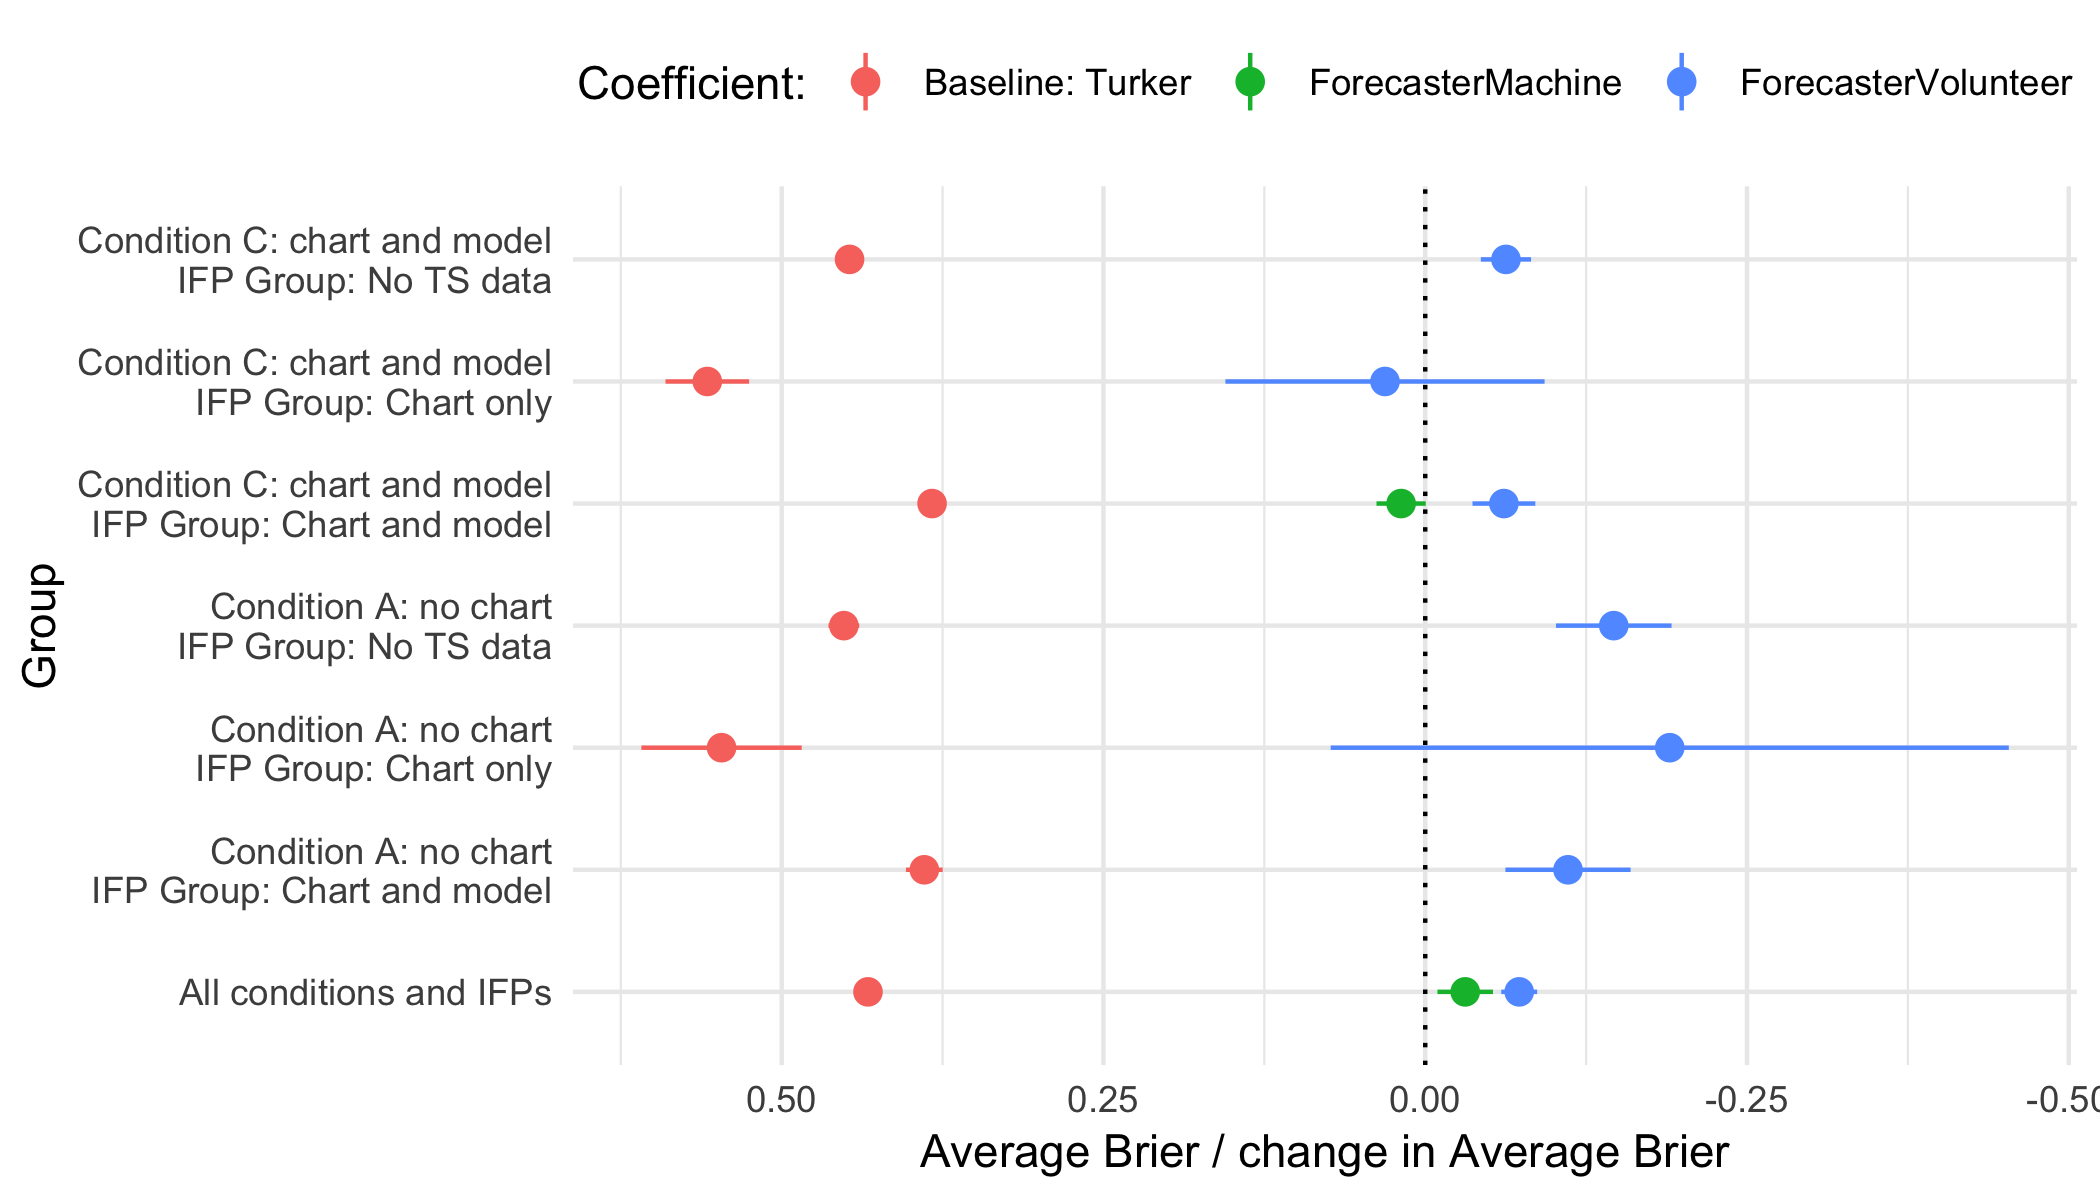
\includegraphics{../output/figures/pairwise-comparisons-turker.png}
\end{figure}

In most groups volunteers have an advantage sufficient to generate
p-values below 0.05, although the effects are minute in comparison to
general between-forecaster differences: all models have very small
adjusted R\^{}2 values, below 0.01.

\subsection{Chart and model effects}\label{chart-and-model-effects}

Teasing out the chart and model effects is a bit harder through pairwise
comparison. Instead, we directly coded whether a forecaster saw a chart
or model forecast. Forcasters in conditions B and C and for questions
that had a chart saw a chart, and forecasters in condition C looking at
a question which had a machine forecast will have seen a model forecast.
We also leave out the machine forecasts from the data, leaving almost
47,000 forecasts, of which about 25\% were made with a chart available,
and 21\% also had a model forecast available.

We estimated two linear models to predict Brier scores for a forecast.
The first has the specifiction:

\[
\begin{aligned}
\textrm{Brier} =~& \alpha + \beta_1\textrm{SeesModel} + \beta_2\textrm{SeesChart} + \beta_3\textrm{IFPGroupChartOnly} + \beta_4\textrm{IFPGroupChartAndModel} \\
 & + \beta_5\textrm{ForecasterVolunteer} 
\end{aligned}
\]

All variables are dummy terms. The intercept \(\alpha\) corresponds to
the average Brier score for a Turker forecasting on an IFP that did not
have chartable data, and who neither saw a chart nor machine forecast.

The second model includes random intercepts for IFP to account for the
possibility that seeings charts or models may make users differentially
willing to forecast on harder IFPs, i.e.~those with higher average Brier
scores. Otherwise the specification of covariates is the same.

\[
\begin{aligned}
\textrm{Brier} =~& \alpha_{\textrm{Global}} + \alpha_{\textrm{IFP}} + \beta_1\textrm{SeesModel} + \beta_2\textrm{SeesChart} + \beta_3\textrm{IFPGroupChartOnly}  \\
 & + \beta_4\textrm{IFPGroupChartAndModel} + \beta_5\textrm{ForecasterVolunteer} 
\end{aligned}
\]

Figure \ref{fig:model-chart-and-model-effects} plots the coefficient
estimates from both models. The results are consistent. Seeing a chart
slightly helps, seeing a model slightly hurts forecast performance.
However, the effects are small and not as important as whether a
forecasters was a volunteer or turker. In addition, the models
themselves capture only a small portion of the variation in Brier scores
overall. Table \ref{tab:model-summary-stats} shows \(R^2\) statistics
for both models. The covariates account for less than 0.01 of the
variation in Brier scores; the inclusion of random IFP intercepts in
model 2 increases this to 0.28 (conditional \(R^2\)), but the fraction
explained by the covariates together is still 0.01 (marginal \(R^2\)).
Most of the variation remains either between forecasters or due to other
random factors.

Thus, while we find that exposure to charts and model forecasts has a
small impact on forecast quality, the effect sizes are small in
comparison to other systematic factors in the model, and small relative
to unsystematic and random factors not in the model.

\begin{figure}
\caption{\label{fig:model-chart-and-model-effects} Model estimates for the direct effects of seeing a chart and machine forecast.}
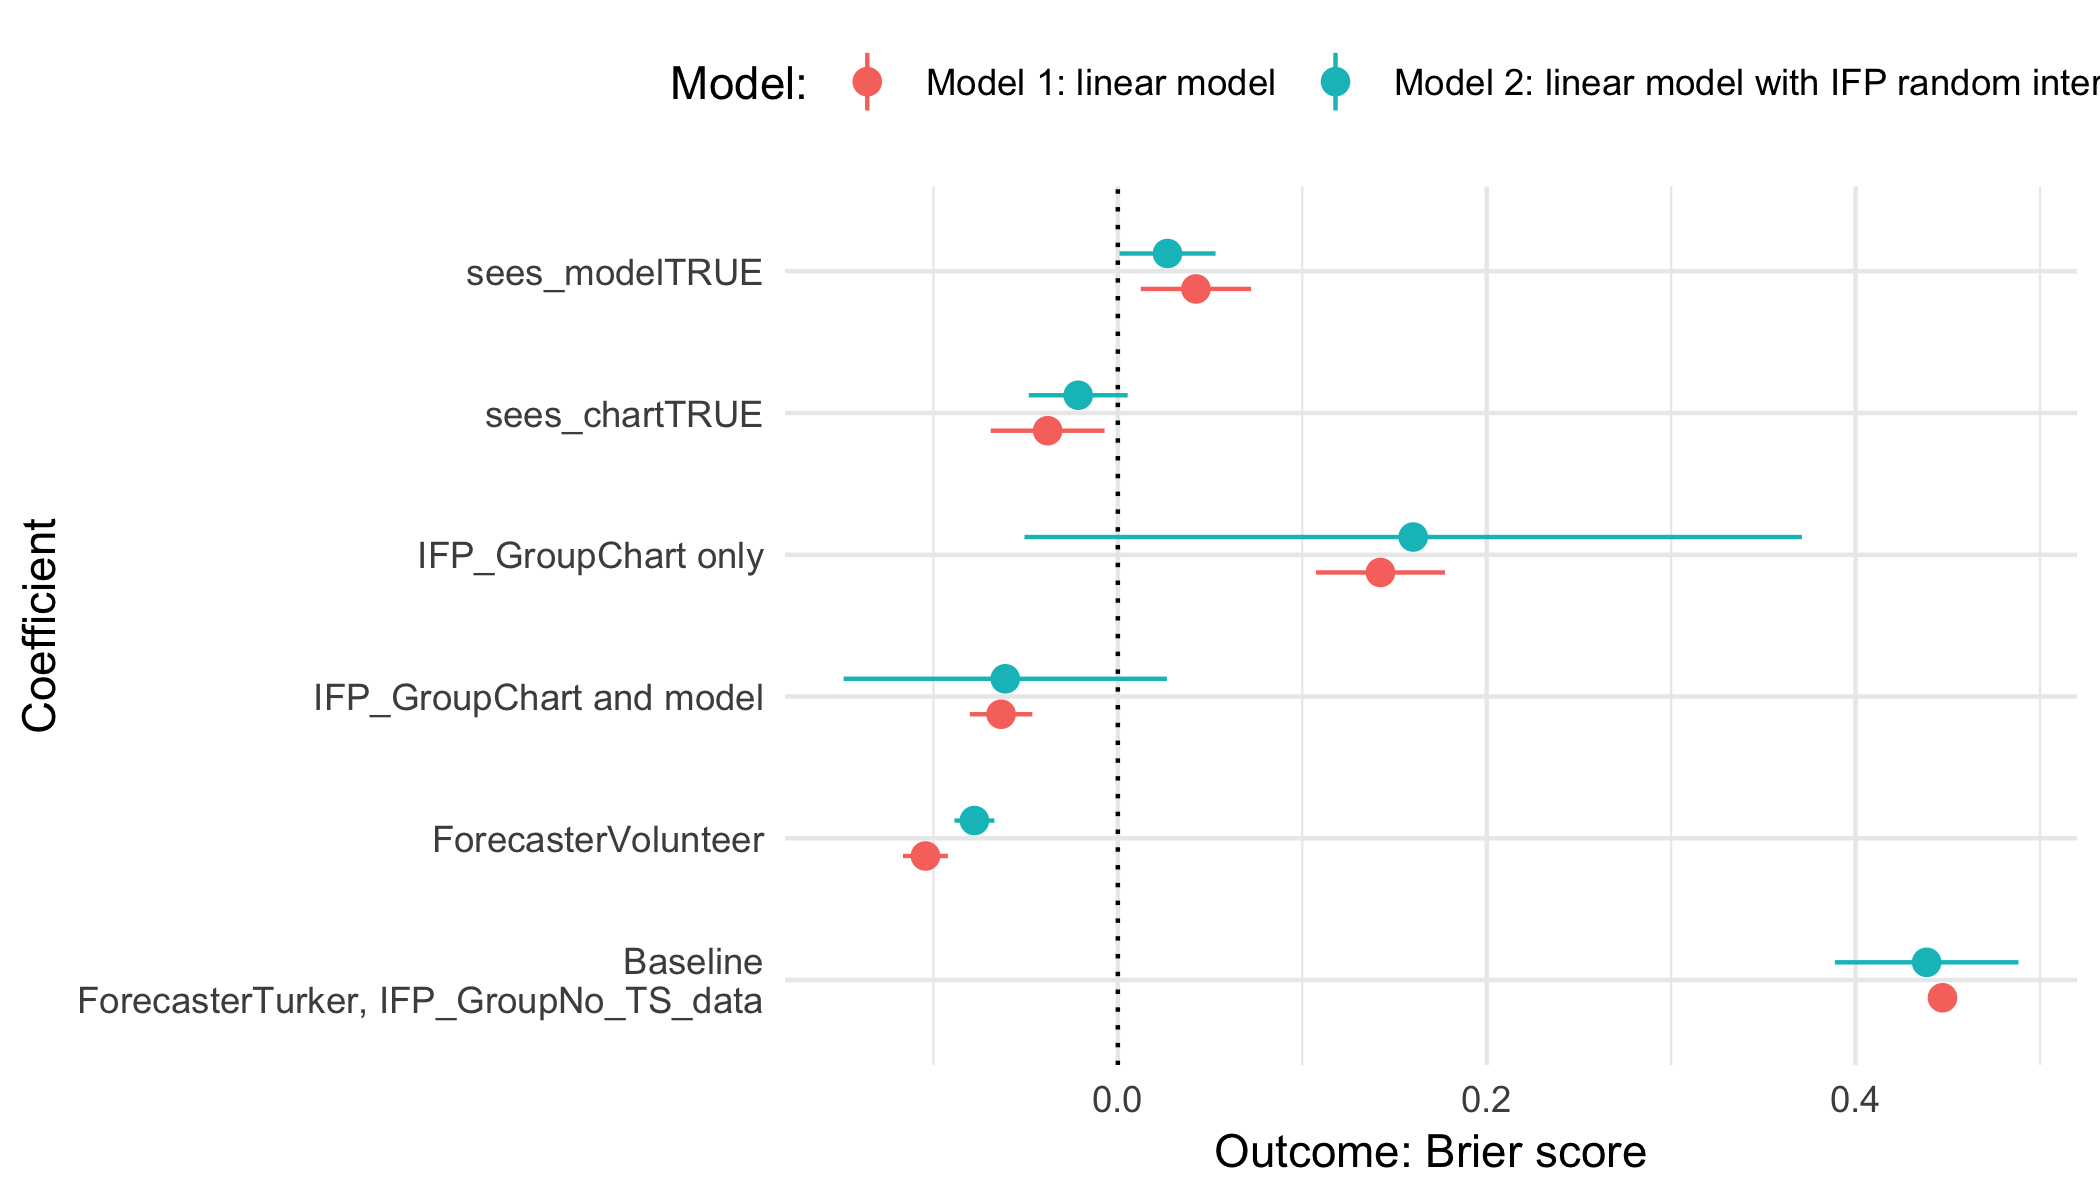
\includegraphics{../output/figures/model-chart-and-model-effects.png}
\end{figure}

\begin{table}

\caption{\label{tab:model-summary-stats}Model summary statistics}
\centering
\begin{tabular}[t]{llr}
\toprule
Model & Statistic & Value\\
\midrule
Model 1: Linear model & N & 46956\\
 & $R^2$ & 0.01\\
 & Adj. $R^2$ & 0.01\\
Model 2: Linear model with IFP random intercepts & N & 46956\\
 & Marginal $R^2$ & 0.01\\
 & Conditional $R^2$ & 0.28\\
\bottomrule
\end{tabular}
\end{table}

\subsection{Models generally were disappointing, but did they do well in
certain
areas?}\label{models-generally-were-disappointing-but-did-they-do-well-in-certain-areas}

Although the machine models overall underperformed, it is possible that
they performed well relative to human forecasters in certain areas. To
examine this we looked at all forecasts for questions that had a machine
forecast. This leaves us with 15,995 forecasts, approximately 2,000 of
which were machine and volunteer forecasts, respectively, and the
remaining 12,000 from turkers.

To estimate the relative performance of different forecasters, we again
estimated a simple linear model, similar to those used for the turker
pariwise comparisons. The model has the general form:

\[
\begin{aligned}
\textrm{Brier} =~& \beta_{i}\textrm{DataSource} + \beta'_{ij}(\textrm{DataSource}\times\textrm{Forecaster})
\end{aligned}
\]

Data source is a discrete variable with \(i=14\) levels for the
different data sources reflected in the set of IFPs. Based on previous
exploratory analysis, we separated one data source, ACLED questions, by
whether a question was binary with two answer options (``yes''/``no''),
or not (3 or 5 options). Forecaster is also a discrete variable with 3
levels, but we leave out ``Machine'' as reference category, giving us
\(j=2\) different levels. Thus, each of the \(\beta\) coefficients
corresponds to the average Brier score for machine forecasts for that
group of IFPs, and each \(\beta'_i\) coefficient is the relative
difference of the average volunteer and turker Brier score compared to
the corresponding baseline in \(\beta_i\).

\begin{figure}
\caption{\label{fig:model-machine-by-data-source} Linear model estimates for the relative performance of machine to volunteer and turker forecasts by data source. The left panel shows the baseline machine performance for each data source, the right panel shows the relative difference of the volunteer and turker forecasts to the corresponding baseline. The outcome variable is a forecasts's Brier score.}
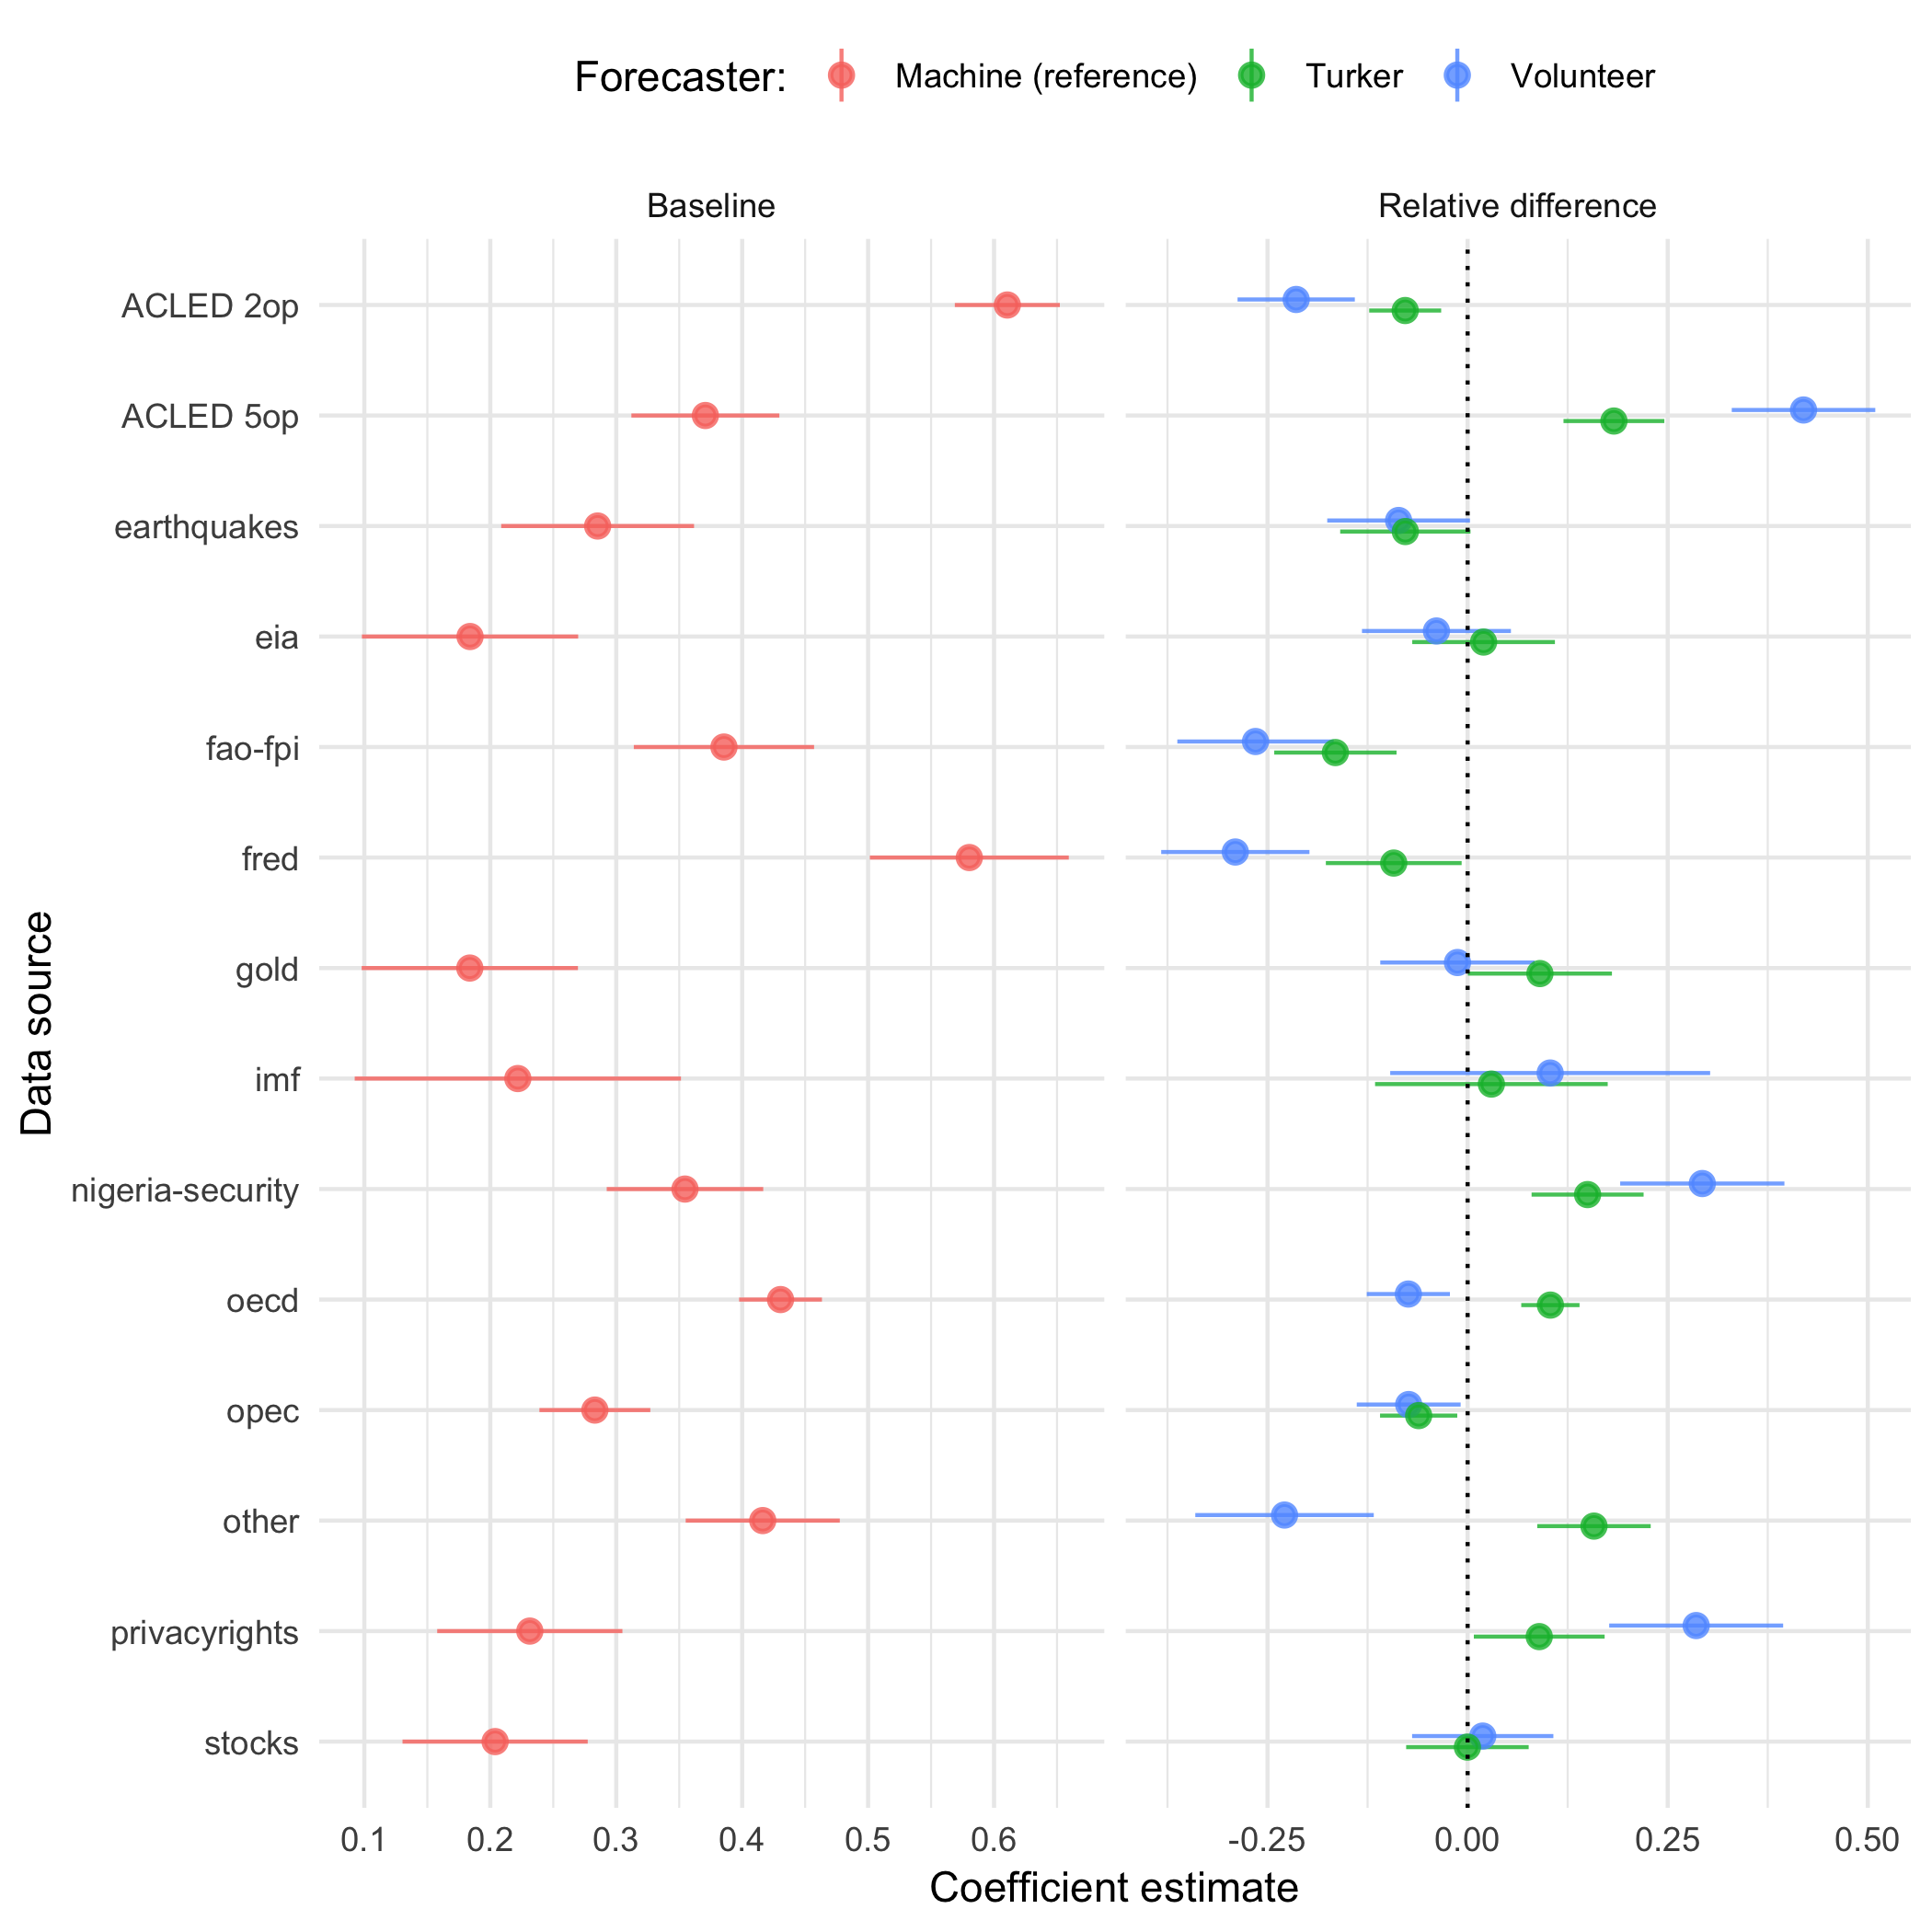
\includegraphics{../output/figures/model-machine-by-data-source.png}
\end{figure}

Figure \ref{fig:model-machine-by-data-source} shows the coefficient
estimates. The left panel shows the baseline machine forecast
performance. The right panel shows the relative difference in average
Brier scores for turker and volunteer forecasts; points to the left of
the dotted 0 line indicate that volunteer or turker forecasters on
average outperformed the machine forecasts.

The machine forecasts did better than human forecasts on ACLED 5-option,
Boko Haram killings (``nigeria-security''), and hacking
(``privacyrights'') questions. All three data sources consist of count
data derived from original event datasets, i.e.~they require data
aggregation before one can see a time series relevant to the question at
hand, which might be a factor in the relative performance on these
questions. On the other hand, human forecasters consistently did better
on ACLED 2-option, food price index (``FAO-FPI''), financial (``fred''),
and oil production (``opec'') questions. The results for ACLED 2-option
questions might be influenced by the particular mechanism by which time
series forecasts were converted to answer option probabilities, which
may explain the inconsistency with ACLED 5-option questions.

There are some hard to quantify factors that may explain some of the
variation in human to machine performance:

\begin{enumerate}
\def\labelenumi{\arabic{enumi}.}
\tightlist
\item
  As mentioned, some data sources (ACLED, privacyrights,
  nigeria-security) required relatively complicated data aggregation to
  derive usable count series, and which therefore may not have been
  accessible to all human forecasters.
\item
  Not all data sources are equally easy to automatically download and
  update, and at least in some of the data sources it was the case that
  models had to forecast over much longer time horizons due to outdated
  data, while a human forecaster would have been able to access more
  recent data.
\item
  Due to obstacles in data acquisition, in at least one case--OPEC oil
  production rates--a secondary and less accurate source was
  substituted. OPEC production values are delivered in monthly PDF
  reports that are difficult to automatically extract data from, and the
  alternative data source in some instances significantly deviated from
  the OPEC values. Thus models for these questions would have been
  forecasting with incorrect input data.
\item
  For questions in which the data source is at a monthly (or higher)
  resolution, humans have an advantage over univariate time series
  models in that they can incorporate sub-monthly information into their
  forecast. For many of these questions, if they were open for a period
  of one or two months, there would in fact have only been one or two
  distinct time series forecasts (barring practical live system issues
  and bugs).
\end{enumerate}

A caveat to these trends is that the number of IFPs and forecasts for
each data source are small and the results may thus be due to random
variation. Results from future RCTs should test this.

\subsection{Why did condition B volunteers do so
well?}\label{why-did-condition-b-volunteers-do-so-well}

Condition B volunteers had the best overall performance out of the 16
groups shown in Table \ref{tab:brier-by-forecaster-ifp-group-condition}.
Considering that the machine forecasts were relatively bad, one possible
explanation is that the charts overall had a positive impact on human
forecast accuracy, while seeing machine forecasts had a negative impact.

However, there are several additional patterns that are either
inconsistent with this simple explanation or at least suggest the need
for a more complex alternative. The first is that condition B
forecasters did not only do better than other groups on questions that
had a chart, but also on questions that did not have a chart. Table
\ref{tab:b-advantage} shows the relevant rows from the average Brier
scores for all forecaster groups in Table
\ref{tab:brier-by-forecaster-ifp-group-condition}. With the partial
exception of the few chart-only questions, condition B forecasters'
advantage on questions without a chart is as pronounced as their
advantage in questions that did have a chart. Considering that there
were two to three times as many forecasts on questions without chartable
data, most of the condition B volunteer advantage is driven by doing
better on questions that did not have a chart.

\begin{table}

\caption{\label{tab:b-advantage}Condition B advantage}
\centering
\begin{tabular}[t]{rllrrr}
\toprule
Group & Condition & IFP\_Group & avg\_Brier & sd\_Brier & n\\
\midrule
7 & B: chart only & No TS data & 0.26 & 0.48 & 1702\\
4 & A: no chart & No TS data & 0.31 & 0.54 & 510\\
13 & C: chart and model & No TS data & 0.38 & 0.60 & 3090\\
\addlinespace
8 & B: chart only & Chart only & 0.42 & 0.42 & 57\\
5 & A: no chart & Chart only & 0.36 & 0.46 & 18\\
14 & C: chart and model & Chart only & 0.59 & 0.57 & 73\\
\addlinespace
9 & B: chart only & Chart and model & 0.23 & 0.31 & 973\\
6 & A: no chart & Chart and model & 0.28 & 0.34 & 274\\
15 & C: chart and model & Chart and model & 0.32 & 0.40 & 1119\\
\bottomrule
\end{tabular}
\end{table}

We could exlain this if there is, in addition to the direct beneficial
effect of seeing a chart, but not a potentially misleading machine
forecast, a spillover effect whereby exposure to charts also improves a
volunteer forecaster's ability to forecast on other questions without
charts.

Curious inconsistencies remain:

\textbf{There appears to be no chart spillover effect for condition C
human and volunteer forecasters.} Tabe
\ref{tab:brier-by-forecaster-ifp-group-condition} shows that condition C
volunteers did worse on questions without time-series data than the
condition A control group. Condition C turkers also did not do better
than their condition A control group counterparts. Unlike condition B
forecasters, they were exposed to machine forecasts as well, so maybe
there is an equal but opposite negative machine spillover effect.

\textbf{Condition B volunteers who forecast a lot do no better on
non-chart questions than novices.} Figure
\ref{fig:cond-b-volunteers-n-vs-brier} show average Brier scores as a
function of the total number of forecasts a user has. The data consist
of only forecasts from condition B volunteers. Each point is the average
Brier score for a user's forecasts on the set of questions that did
(blue) or did not have a chart (red). Novice users tend to be as
accurate as intensive users on non-chart questions. This implies that
the condition B volunteer advantage on non-chart questions is not
related to how active a user was. If there is a spillover effect, even
very inactive users seem to somehow benefit from it.

\begin{figure}
\caption{\label{fig:cond-b-volunteers-n-vs-brier} Average Brier for condition B volunteers by user and by whether a IFP had a chart. Intensive users are slightly more accurate than novice users on questions with a chart, but no more accurate on questions without a chart.}
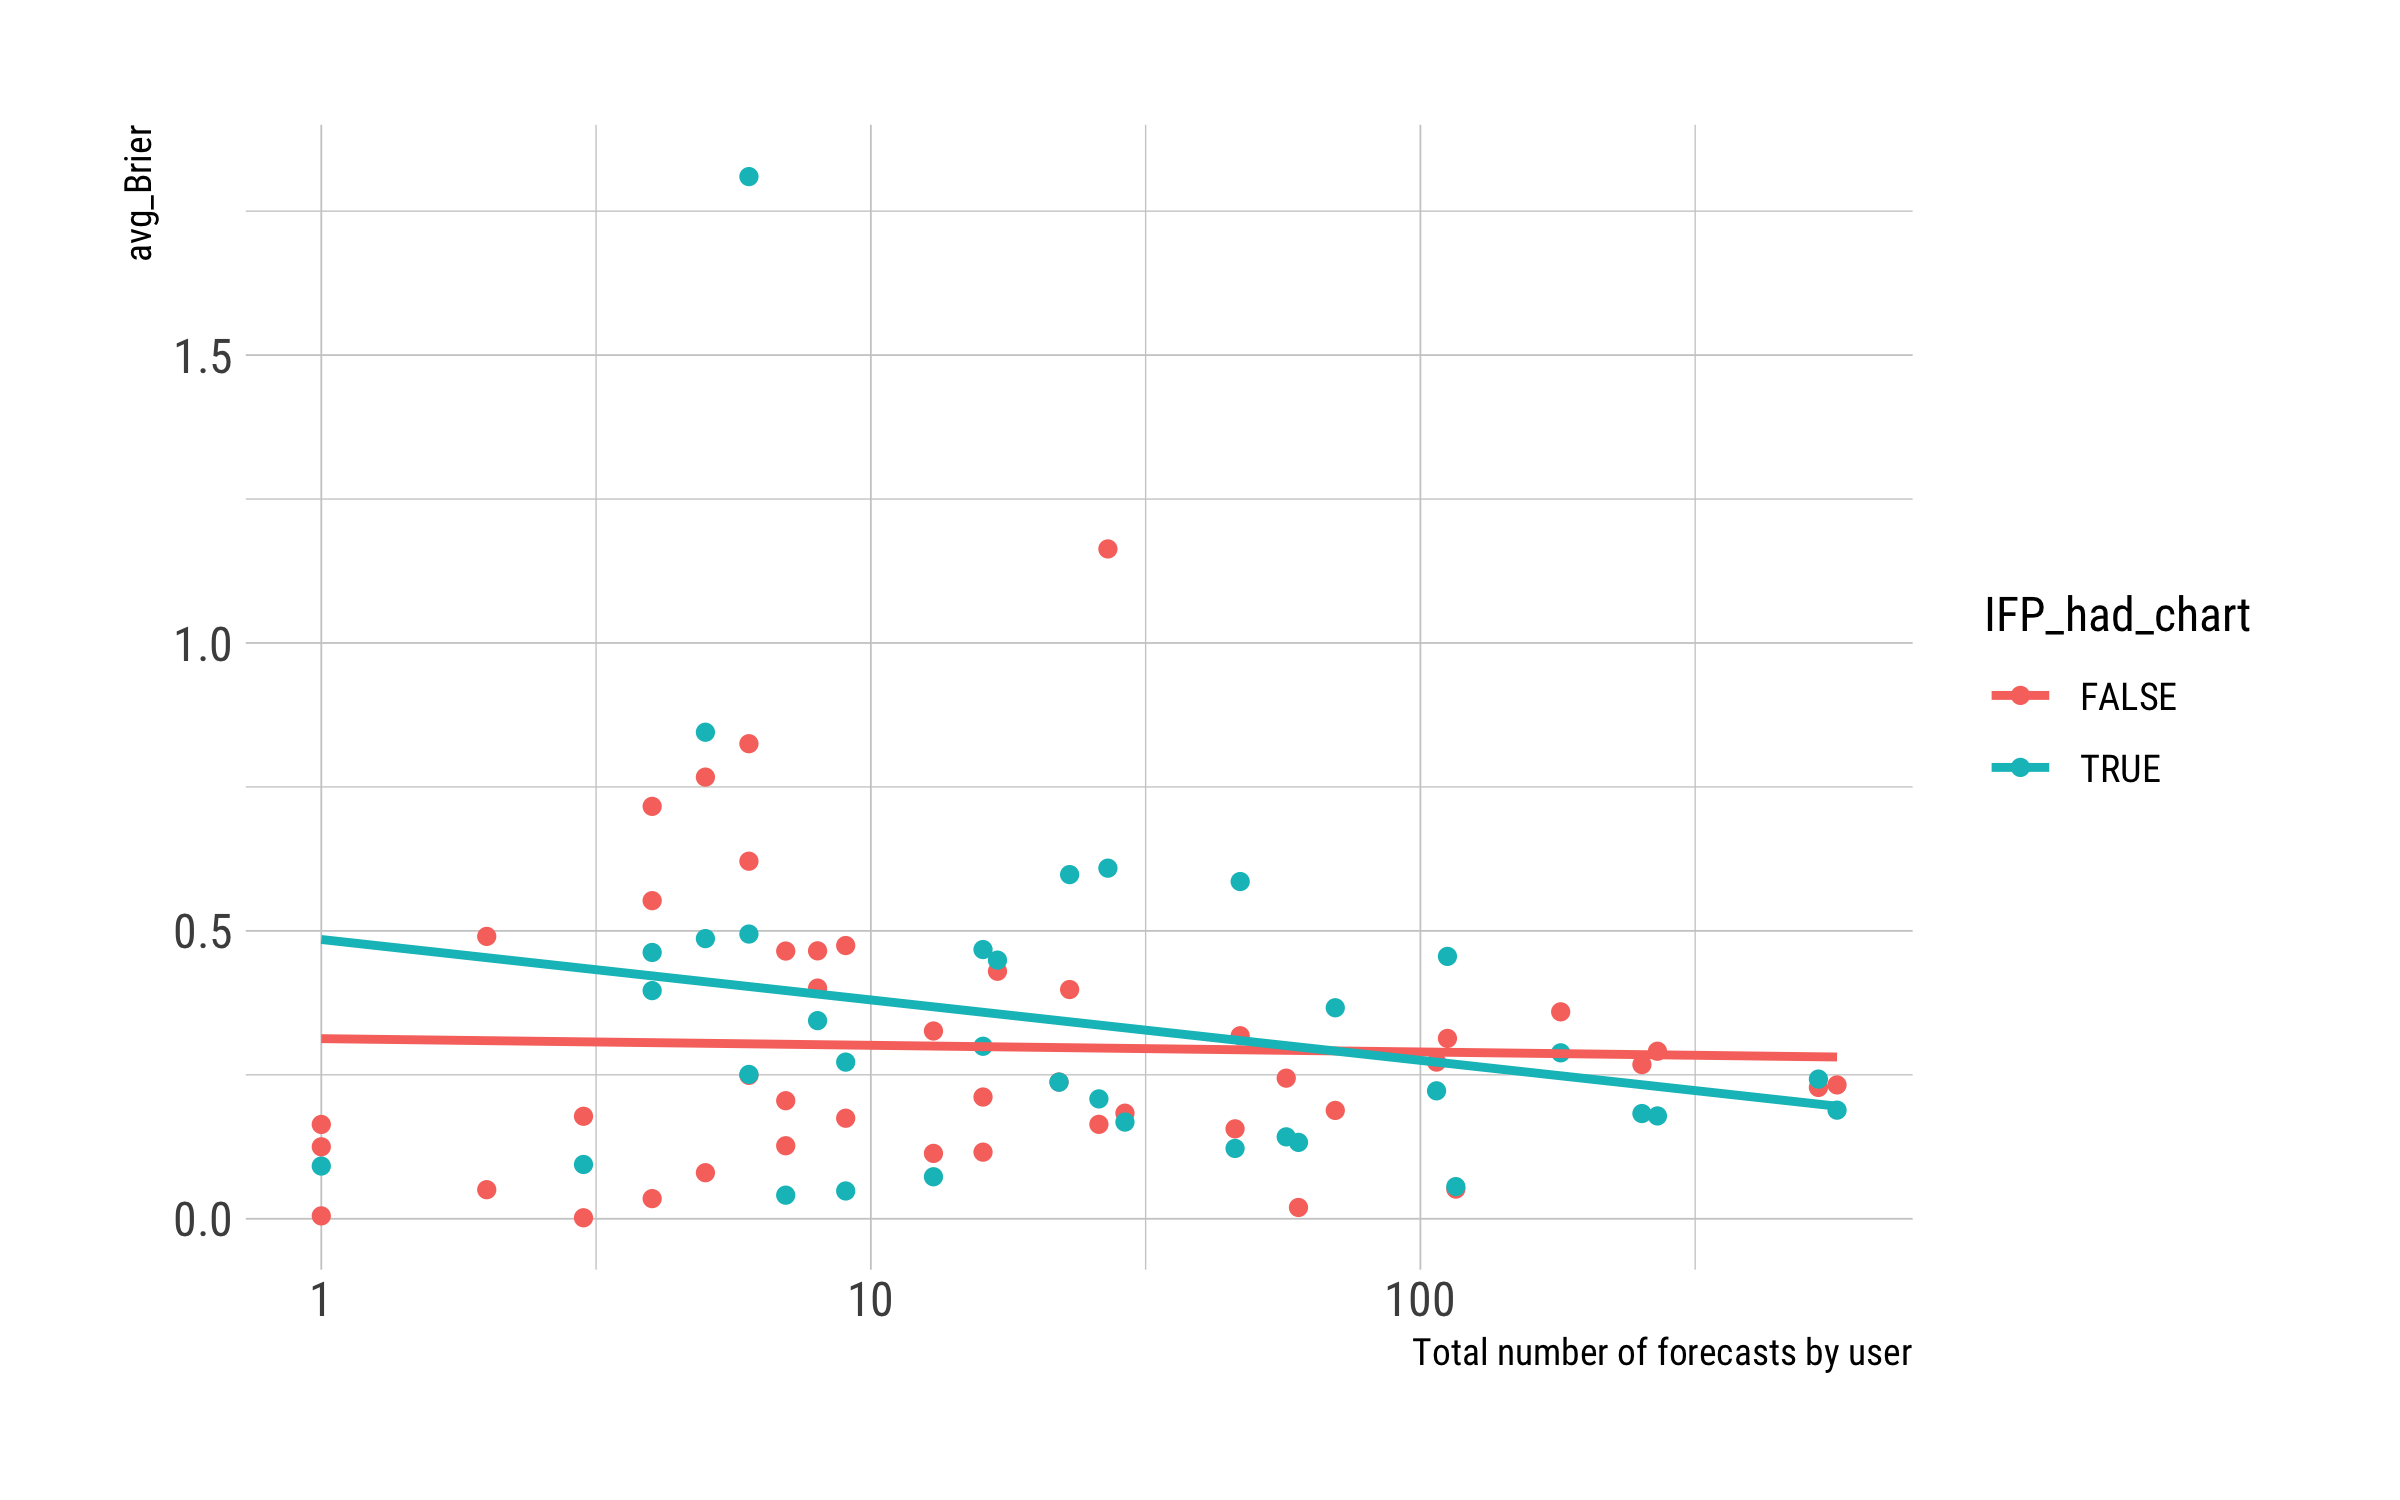
\includegraphics{../output/figures/cond-b-volunteers-n-vs-brier.png}
\end{figure}

\textbf{Condition C volunteers do well on questions where we know that
data displayed was wrong.} There were several instances where we know
that the data displayed in a chart were inaccurate. Figure
\ref{fig:iraq} shows the first example, oil production figures for Iraq.
The main chart shows several teim series depicting oil production in
Iraq, according to different sources. The canonical data are contained
in monthly OPEC oil market reports, each of which contains production
figures for the past 3 months. Those are shown in the sequence of short
time series on the mid-right part of the main chart--the figures are
somewhat inconsistent between reports, but this is another peculiarity.
Because this data is difficult to obtain programatically, an alternative
data source is used instead. This is what would have been shown in the
charts, and what informed the machine forecast. Obviously it is
incorrect data. The dotted lines show the values separating the answer
options for this question. The chart placed the production values in an
entirely incorrect answer category.

\begin{figure}
\caption{\label{fig:iraq} Iraq oil production}
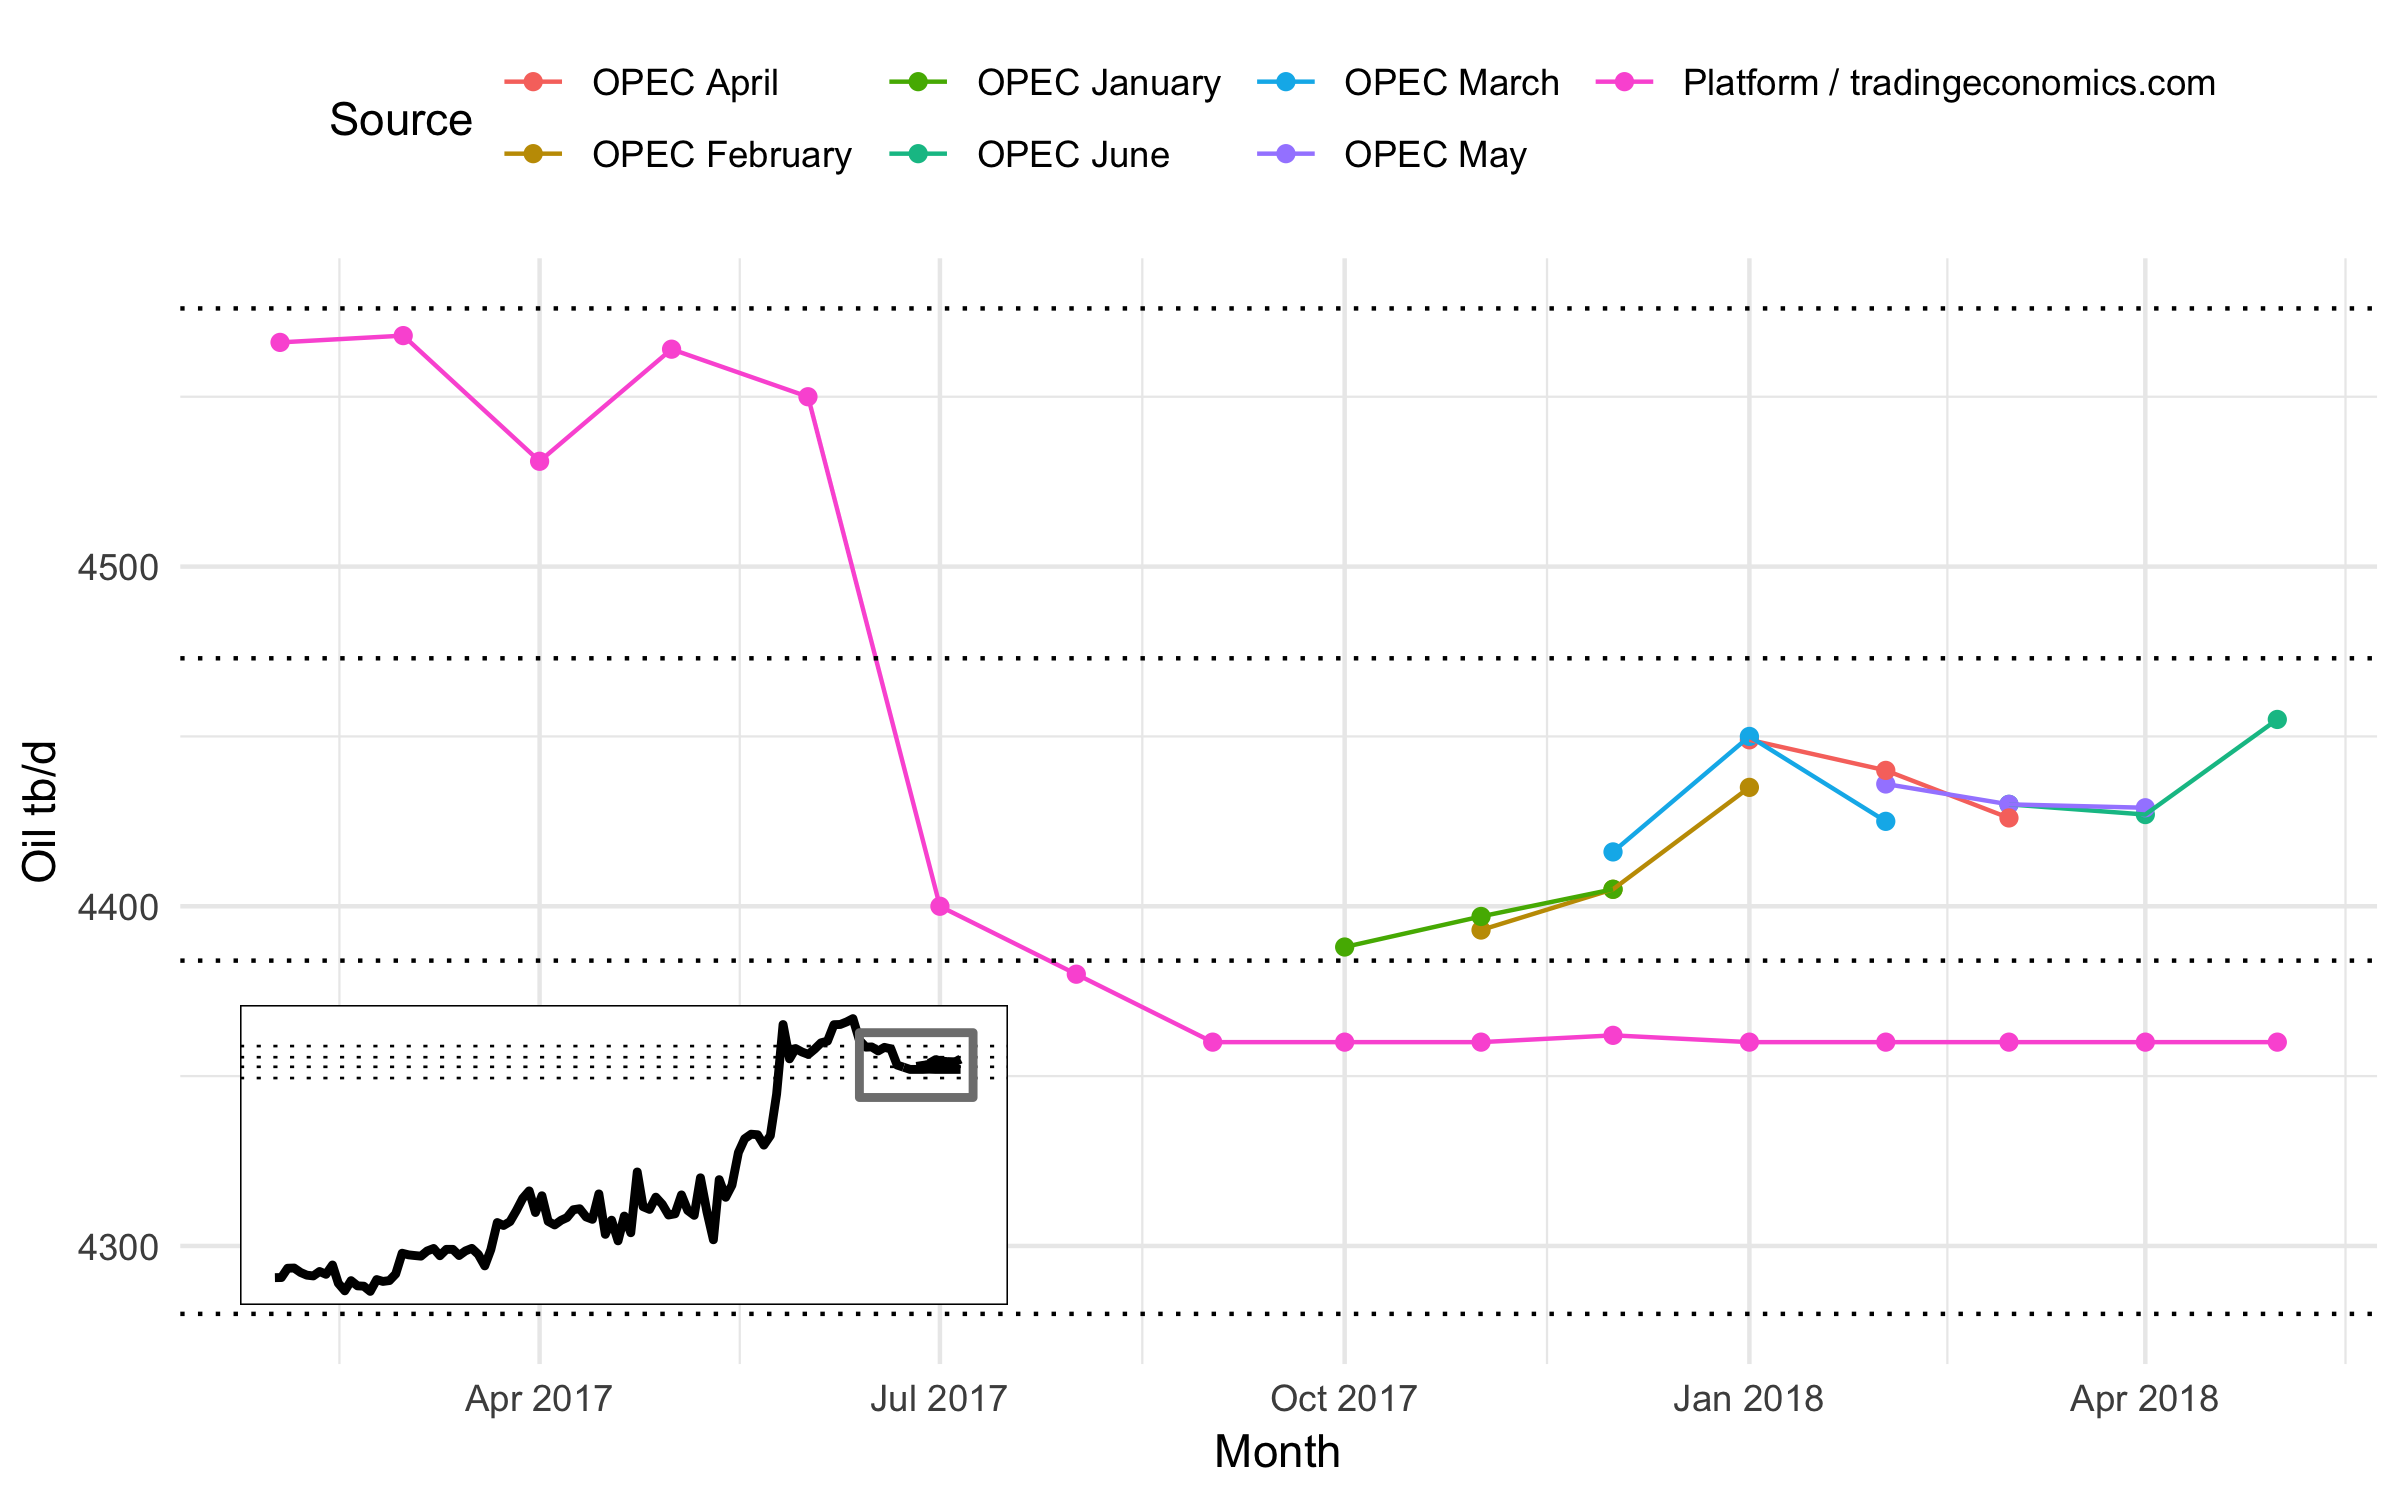
\includegraphics{../output/figures/opec-iraq-divergence.png}
\end{figure}

Curiously, the condition B volunteers performed better on this question
than any other forecaster. The number of forecasts here are low, and
only the last three groups, starting from the machine forecasts, have
pairwise statistically significant differences in average Brier score
from the condition B volunteers.

\begin{longtable}[]{@{}llrr@{}}
\toprule
Forecaster & condition & avg\_Brier & n\tabularnewline
\midrule
\endhead
Volunteer & b & 0.07 & 5\tabularnewline
Volunteer & a & 0.11 & 5\tabularnewline
Turker & c & 0.18 & 87\tabularnewline
Machine & n/a & 0.25 & 14\tabularnewline
Turker & a & 0.35 & 23\tabularnewline
Volunteer & c & 0.45 & 21\tabularnewline
\bottomrule
\end{longtable}

Another example with incorrect data is an early ICEWS question that fell
outside the common period and thus did not have forecasts from turkers.
Condition B volunteers also outperformed all other groups on this
question, although the pairwise differences with the other groups are
not statistically significant.

\begin{longtable}[]{@{}llrr@{}}
\toprule
Forecaster & condition & avg\_Brier & n\tabularnewline
\midrule
\endhead
Volunteer & b & 0.92 & 14\tabularnewline
Machine & n/a & 1.00 & 18\tabularnewline
Volunteer & a & 1.11 & 7\tabularnewline
Volunteer & c & 1.11 & 25\tabularnewline
\bottomrule
\end{longtable}

\clearpage

\textbf{Even when the machine predictions were good, condition B
volunteers did better than their C counterparts.} If bad machine
predictions influence human forecasts and are the reason why the
beneficial chart effecgt is only apparent in condition B forecasters,
and not condition C forecasters, then it should also be the case that
condition C forecasters do well on those questions where the machine
forecasts were good. This is no the case. The table below shows the
subset of forecasts on questions that had a machine forecast (and thus
chart) and where the machine forecast average Brier was lower than the
average Brier score for the forecasts from all other forecaster
\(\times\) condition groups. Condition B volunteers beat their condition
C counterparts even when the machine model should have improved their
forecasts because they happened to be accurate.

\begin{longtable}[]{@{}llrr@{}}
\toprule
Forecaster & Condition & avg\_Brier & n\_fcasts\tabularnewline
\midrule
\endhead
Machine & Machine & 0.39 & 1975\tabularnewline
Turker & A: no chart & 0.39 & 2810\tabularnewline
Turker & C: chart and model & 0.38 & 8482\tabularnewline
Volunteer & A: no chart & 0.28 & 267\tabularnewline
Volunteer & B: chart only & 0.23 & 958\tabularnewline
Volunteer & C: chart and model & 0.32 & 1094\tabularnewline
\bottomrule
\end{longtable}

One possibility that we should not discard with these apparent
inconsistencies is that we are digging in noise. All of the
effects---for turkers versus other forecasts, for the disappointing
performance of the machine forecasts, for conditions or different
groupings of IFPs---pale in comparison to differences in accuracy
between individual forecasters and between forecasts for different IFPs.
But on the other hand there are several inconsistencies so it also is a
stretch to write all of them off to random coincidence. Condition B
volunteers clearly did better than all other forecasters/condition
groups, but it is not clear why.

\section{Conclusion}\label{conclusion}

Are we digging in noise?

Many of the questions involve monthly time series but are only open for
periods spanning a single or few months. Some of the advantage of the
human forecasters may thus have been due to operating on a sub-monthly
time scale.

We also know that model performance suffered from issues related to
automation. Were we able to run the RCT-A questions with the current
system and with a data platform that optimally ingests data sources on
the bleeding edge of their own updates, our forecasts would have been
\ldots{}

\textbf{{[}check with updated results from test bed what the performance
gain would have been, i think the site visit stats were not accurate
anymore{]}}

\section{Additional information}\label{additional-information}

\begin{longtable}[]{@{}lrrrr@{}}
\caption{Average Brier scores for machine and other forecasts by
question data source.}\tabularnewline
\toprule
Data\_source & N\_IFPs & Machine & Turker & Volunteer\tabularnewline
\midrule
\endfirsthead
\toprule
Data\_source & N\_IFPs & Machine & Turker & Volunteer\tabularnewline
\midrule
\endhead
ACLED 2op & 7 & 0.611 & 0.533 & 0.396\tabularnewline
ACLED 5op & 4 & 0.371 & 0.554 & 0.790\tabularnewline
earthquakes & 2 & 0.285 & 0.207 & 0.199\tabularnewline
eia & 5 & 0.184 & 0.204 & 0.145\tabularnewline
fao-fpi & 3 & 0.386 & 0.220 & 0.121\tabularnewline
fred & 2 & 0.580 & 0.488 & 0.290\tabularnewline
gold & 3 & 0.184 & 0.274 & 0.171\tabularnewline
imf & 1 & 0.222 & 0.252 & 0.325\tabularnewline
nigeria-security & 2 & 0.355 & 0.504 & 0.648\tabularnewline
oecd & 7 & 0.430 & 0.534 & 0.356\tabularnewline
opec & 5 & 0.283 & 0.222 & 0.209\tabularnewline
other & 2 & 0.416 & 0.574 & 0.188\tabularnewline
privacyrights & 2 & 0.231 & 0.321 & 0.517\tabularnewline
stocks & 4 & 0.204 & 0.204 & 0.223\tabularnewline
\bottomrule
\end{longtable}

\section*{References}\label{references}
\addcontentsline{toc}{section}{References}

\hypertarget{refs}{}
\hypertarget{ref-hyndman:khandakar:2008}{}
Hyndman, Rob J., and Yeasmin Khandakar. 2008. ``Automatic Time Series
for Forecasting: The Forecast Package for R.'' \emph{Journal of
Statistical Software} 27 (3). Monash University, Department of
Econometrics; Business Statistics.

\hypertarget{ref-kahneman:2011}{}
Kahneman, Daniel, and Patrick Egan. 2011. \emph{Thinking, Fast and
Slow}. Vol. 1. Farrar, Straus; Giroux New York.

\hypertarget{ref-tetlock:2005}{}
Tetlock, Philip. 2005. \emph{Expert Political Judgment: How Good Is It?
How Can We Know?} Princeton, NJ: Princeton University Press.

\hypertarget{ref-tetlock:etal:2017}{}
Tetlock, Philip E, Barbara A Mellers, and J Peter Scoblic. 2017.
``Bringing Probability Judgments into Policy Debates via Forecasting
Tournaments.'' \emph{Science} 355 (6324). American Association for the
Advancement of Science: 481--83.


\end{document}
